\documentclass[12pt,a4paper]{article}
\usepackage{amsmath}
\usepackage{amsfonts}
\usepackage{amssymb}
%\usepackage{polski}
\usepackage{indentfirst}
\usepackage{graphicx}
\usepackage{placeins}
\usepackage{verbatim}
\usepackage[hidelinks]{hyperref}
\usepackage{graphics}
\graphicspath{ {./images/} }


% Default fixed font does not support bold face
\DeclareFixedFont{\ttb}{T1}{txtt}{bx}{n}{12} % for bold
\DeclareFixedFont{\ttm}{T1}{txtt}{m}{n}{12}  % for normal

% Custom colors
\usepackage{color}
\definecolor{deepblue}{rgb}{0,0,0.5}
\definecolor{deepred}{rgb}{0.6,0,0}
\definecolor{deepgreen}{rgb}{0,0.5,0}

\usepackage{listings}

% Python style for highlighting
\newcommand\pythonstyle{\lstset{
language=Python,
basicstyle=\ttm,
morekeywords={self},              % Add keywords here
keywordstyle=\ttb\color{deepblue},
emph={MyClass,__init__},          % Custom highlighting
emphstyle=\ttb\color{deepred},    % Custom highlighting style
stringstyle=\color{deepgreen},                     % Any extra options here
showstringspaces=false
}}


% Python environment
%\begin{python}
%\end{python}
\lstnewenvironment{python}[1][]
{
\pythonstyle
\lstset{#1}
}
{}

% Python for external files
%\pythonexternal{xxx.py}
\newcommand\pythonexternal[2][]{{
\pythonstyle
\lstinputlisting[#1]{#2}}}

% Python for inline
%\pythoninline{xxxxx}
\newcommand\pythoninline[1]{{\pythonstyle\lstinline!#1!}}



\newcommand\todo[1]{\textcolor{red}{#1}}
\usepackage[utf8]{inputenc}
\begin{document}

\title{
  Kryptografia - Algorytm ElGamal \\
   sposób działania i implementacja \\
    \small na podstawie \textit{"A Public Key Cryptosystem and a Signature
Scheme Based on Discrete Logarithms, 
TAHER ELGAMAL"}}

\author{
  Adamski, Wojciech\\
  \texttt{242359}
  \and
  Górska, Kinga\\
  \texttt{259505}
  \and
  Mochoń, Filip\\
  \texttt{259480}
}
\date{19 Maja 2022}
\maketitle
\tableofcontents
\newpage
%początek sekcji pierwszej
\section{Wprowadzenie - Co to jest algorytm ElGamala}
Algorytm \textbf{ElGamal} to jeden z najważniejszych algorytmów kryptografii asymetrycznej. Opiera się on o trudność rozwiązania algorytmu dyskretnego w ciele liczb całkowitych modulo dużych liczb pierwszych. Jego nazwa pochodzi od egipskiego kryptografa \textbf{Tahera Elgamala} w latach 80. $XX$w. Algorytm ten jest wykorzystywany między innymi do podpisów cyfrowych, ale różne jego modyfikacje mogą służyć do wielu innych zastosowań.
\section{Klucz Publiczny}\
\begin{itemize}
\item $x_{A}$  - klucz tajny A 
\item $x_{B}$ - klucz tajny B  
\item p - duża liczba pierwsza (znane)
\item $\alpha$ - element w ciele p (znane)
\end{itemize}
 Strona A oblicza: 
 
     \[y_{A} \:\equiv\: \alpha^{x_{A}}\, mod\, p \]

 i wysyła $y_{A}$. Podobnie, B oblicza $y_{B} \:\equiv\: \alpha^{x_{B}}\, mod\, p$ i je wysyła.
 Wtedy $K_{AB}$ jest obliczane: 
 \[K_{AB}\:\equiv\:\alpha^{x_{A}x_{B}}\,mod\,p\]
   \[ \equiv y_{A}^{x_{B}}\,mod\,p\]
 \[\equiv y_{B}^{x_{A}}\,mod\,p\]
 Zarówno strona A jak i B potrafi obliczyć $K_{AB}$. Nadal nie udowodniono, że złamanie systemu polega na obliczeniu logarytmu dyskretnego. \\
 Dobranie odpowiedniego p polega na tym, że $p-1$ posiada przynajmniej jeden duży dzielnik pierwszy.\\
 Przypuśćmy, że A chce wysłać wiadomość $m$ do B (gdzie $0 \leq m \leq p-1$). Najpierw A wybiera k z przedziału $(0,p-1)$, a następnie oblicza klucz:
 \begin{gather}
    K\equiv y_{B}^{k}\,mod\,p 
 \end{gather}
 
 $y_{B}$ A dostaje od B lub jest publiczne. Zaszyfrowana wiadomość jest krotką $(c_{1}, c_{2})$, gdzie:
 \begin{gather}
     c_{1} \equiv \alpha^{k}\,mod\,p\;\:\:\:\:\;c_{2} \equiv Km\,mod\,p
 \end{gather}
 
 \\
 Deszyfrowanie rozbija się na dwie części. Najpierw trzeba odzyskać $K$ \[K\equiv (\alpha^{k})^{x_{B}}\equiv c_{1}^{X_{B}}\,mod\,p\]
 $x_{B}$ jest znane tylko B. Drugim krokiem jest rozszyfrowanie $c_{2}$
 \\
 Nierekomendowane jest używanie tej samej wartości $k$ do szyfrowania więcej niż jednego bloku wiadomości, gdyż
 w przypadku złamania $m_{1}$ haker może odszyfrować resztę wiadomości. Załóżmy, że:
 \[c_{1,1}\equiv \alpha^{k}\,mod\,p \:\:\:\:\:\: c_{2,1}\equiv m_{1}K\,mod\,p\]
 \[c_{1,2}\equiv \alpha^{k}\,mod\,p \:\:\:\:\:\: c_{2,2}\equiv m_{2}K\,mod\,p\]
 wtedy $\frac{m_{1}}{m_{2}} \equiv \frac{c_{2,1}}{c_{2,2}}\,mod\,p$, a $m_{2}$ jest łatwe do policzenia jeżeli znane jest $m_{1}$
%początek sekcji drugiej
\section{Schemat podpisu elektronicznego}
\begin{itemize}
    \item $m$ - dokument do podpisania, gdzie $0\leq m \leq p-1$
    \item $y$ - klucz publiczny, gdzie $y \equiv \alpha^{x}\,mod\,p$
    \item $x_{A}$ - klucz prywatny
\end{itemize}
Podpis dla $m$ jest parą $(r,s), 0\leq r,s < p-1$ w taki sposób, że: 
\begin{gather}
   \alpha^{m} \equiv y^{r}r^{s}\,mod\,p \:\:\: 
\end{gather}

\begin{enumerate}
    \item Podpisywanie\\
    \begin{enumerate}
        \item wybierz liczbę $k$ taką, że $0<k<p-1$, a $NWD(k,p-1) = 1$
        \item oblicz: 
            
            \begin{gather}
                r \equiv \alpha^{k}\,mod\,p
                \end{gather}
            
        
        \item teraz można zapisać (3): 
        \begin{gather}
            \alpha^{m} \equiv \alpha^{xr}\alpha^{ks}\,mod\,p
        \end{gather}
        
        \item powyższe równanie można rozwiązać dla $s$:
        \begin{gather}
            m \equiv xr + ks\,mod\,(p-1)
        \end{gather}
        
    \end{enumerate}
    \item Procedura weryfikacji\\
    Posiadając $m, \,r$ i $ s$ łatwo jest zweryfikować autentyczność podpisu poprzez obliczenie obu wartości i sprawdzenie czy są równe.
\end{enumerate}
\section{Przykładowe ataki na schemat podpisu}
W tej części pokazane będą przykładowe możliwości ataku na schemat podpisu. Niektóre ataki polegają na obliczeniu logarytmu dyskretnego na $GF(p)$. Dotychczas jednak nie udowodniono, że złamanie schematu podpisu jest tożsame z obliczeniem logarytmu dyskretnego. Jednakże żadne z tych ataków nie zakończyły się jeszcze złamaniem szyfru. Ataki będą podzielone na dwie grupy. Pierwsza z nich zawiera ataki polegające na odzyskaniu klucza prywatnego $x$, a druga pokazuje niektóre ataki polegające na podrobieniu podpisu bez posiadania $x$.
\begin{enumerate}

    \item Ataki polegające na odzyskaniu $x$:
    % trzeba to dobrze przetłumaczyć bo piszę pierdoły
    \todo{trzeba to dobrze przetłumaczyć bo piszę pierdoły}
    \begin{enumerate}
        \item Atak 1:\\
        Posiadając $\{ m_{i}:\,i=1,2,...,l\}$ dokumentów z odpowiadającymi podpisami $\{r_{i},\,s_{i}:\,i=1,2,...,l\}$ haker może próbować rozwiązać $l$ równań odzyskujących z (6). Ponieważ jest $l+1$ niewiadomych liczba rozwiązań jest ogromna. Powód, dla którego do każdej wartości dla $x$ odpowiada rozwiązanie dla $k_{i}$ jest taki, że są to wartości liniowe macierzy współczynników.
        Jeżeli jakiekolwiek $k$ jest użyte więcej niż raz do podpisu to system równań jest jasno określony i $x$ może zostać odzyskane. 
        \item Atak 2:\\
        Próba rozwiązania równań (3) jest równoważna do obliczenia logarytmu dyskretnego na $GF(p)$, ponieważ obie niewiadome $x$ i $k$ pojawiają się w wykładniku.
        \item Atak 3:\\
        Atakujący mógłby spróbować rozwinąc zależność liniową pośród niewiadomych $\{ k_{i},\,i=1,2,...,l\}$. Wiąże się to z obliczeniem logarytmu dyskretnego, ponieważ jeżeli $k_{i}\equiv ck_{j}\,mod\,(p-1)$, wtedy $r_{i}\equiv r_{j}^{c}\,mod\,p$ i jeżeli $c$ może być obliczone, wtedy rozwiązanie logarytmu dyskretnego jest łatwe.
    \end{enumerate}
    \item Ataki fałszujące podpis
    \begin{enumerate}
        \item Atak 4:\\
        Posiadając dokument $m$ fałszerz mógłby spróbować znaleźć $r,\,s$ takie, że (3) zostałoby spełnione. Jeżeli $r\equiv \alpha^{j}\,mod\,p$ jest ustalone dla danego $j$ (wybranego losowo to obliczenie $s$ jest równoznaczne z rozwiązaniem logarytmu dyskretnego na $GF(p)$.\\
        Jeżeli fałszerz ustali $s$ najpierw, wtedy $r$ może być obliczone z równania 
        \begin{gather}
            r^{s}y^{r} \equiv A\,mod\,p
        \end{gather}
        Rozwiązanie równania (7) dla $r$ jeszcze nie zostało potwierdzone jakoby było równie trudne jak rozwiązanie logarytmu dyskretnego, ale podejrzewa się, że jest niewykonalne obliczenie (7) w wielomianowym czasie. 
        \item Atak 5:\\
        Wydaje się możliwe, że (3) może być rozwiązane dla zarówno $r$ i $s$ jednocześnie, ale nie znaleziono dotychczas odpowiedniego algorytmu.
        \item Atak 6:\\
        Atak na schemat podpisu pozwala na utworzenie fałszywego-prawdziwego podpisu znając jeden z poprzednich prawdziwych podpisów. Atak ten jednakże nie łamie systemu szyfrowania, gdyż nie można tak wygenerowanym podpisem podpisać dowolnej wiadomości.\\
        Jeżeli podpis $(r, s)$ jest prawdziwy dla wiadomości $(m)$, wtedy
        \[\alpha^{m}=y^{r}r^{s}\,mod\,p\]
        Wybierzmy liczby całkowite $A,B$ oraz $C$ takie, że $(Ar-Cs)$ jest względnie pierwsze do $p-1$. Wtedy:
        \[
        r' \equiv r^{A}\alpha^{B}y^{C}\,mod\,p\]
       \[ s'\equiv \frac{sr'}{(Ar - Cs)\,mod\,(p-1)}\]
       \[ m'\equiv\frac{r'(Am+Bs)}{(Ar - Cs)\,mod\,(p-1)}
        \]
        Wtedy zakłada się że $(r`,s`)$ może podpisać wiadomość $(m')$.
        Obliczamy (w ciele $p$):
        \[y^{r'}r'^{s'} \equiv r^{r'}(r^{A}\alpha^{B}y^{C})^{\frac{sr'}{(Ar-Cs}}\]
        \[\equiv(y^{r'Ar-r'Cs+r'Cs}r^{Asr'}\alpha^{Bsr'})^{\frac{1}{(Ar-Cs)}}\]
        \[\equiv((y^{r}r^{s})^{Ar'}\alpha^{Bsr'}^{\frac{1}{(Ar-Cs)}}\]
        \[\equiv\alpha^{\frac{mAr'+Bsr'}{Ar-Cs}}\]
        \[\equiv\alpha^{m'}\]
        W szczególnym przypadku, gdy $A=0$ prawdziwe podpisy mogą być generowane do odpowiadających sobie wiadomości nawet bez znajomości żadnego podpisu:
        \[r'\equiv\alpha^{B}y^{C}\,mod\,p\]
        \[s'\equiv\frac{-r'}{C\,mod\,(p-1)}\]
        \[m'\equiv\frac{-r'B}{C\,mod\,(p-1)}\]
        Widać więc, że $(r', s')$ podpisze wiadomość $(m')$.
    \end{enumerate}
\end{enumerate}
\section{Właściwości systemu ElGamala i porównanie go do innych schematów podpisu i systemu kluczy publicznych.}
Weźmy $m$, które będzie liczbą bitów $p$ dla logarytmu dyskretnego, albo $n$ dla faktoryzacji liczb całkowitych. Wtedy najlepszy znany algorytm do obliczania  logarytmów dyskretnych, jak i faktoryzacji liczb całkowitych (który jest funkcją używaną w niektórych obecnych systemach, na przykład \bold{RSA})
\[O(exp\sqrt{cm\ln{m}})\]
gdzie najlepszym przybliżeniem dla $c$ jest $c=0.69$ dla faktoryzacji liczb całkowitych, jak i dla logarytmów dyskretnych na $GF(p)$. Te założenia sugerują, że musimy używać liczb, które są rozmiarem zbliżone do tych używanych w RSA w celu osiągnięcia podobnego poziomu bezpieczeństwa.  
\begin{enumerate}
    \item Właściwości systemu kluczy publicznych\\
    Jak wykazano powyżej, system ElGamala różni się od innych systemów. Po pierwsze, w celu wdrożenia losowości przy kodowaniu, szyfrogram dla danej wiadomości $m$ jest niepowtarzalny, na przykład jeżeli chcemy zaszyfrować tą samą wiadomość dwa razy, to nie otrzymamy tego samego szyfrogramu $(c_{1}, c_{2})$. To zapobiega atakom polegającym na odgadywaniu fragmentów tekstu, czyli jeżeli atakujący podejrzewa, że dany fragment tekstu to $m$, a potem spróbuje zaszyfrować to $m$ to patrząc na szyfrogram nie będzie w stanie się upewnić czy miał rację, gdyż oryginalny nadawca może użyć innego $k$ i otrzymać zupełnie inny wynik szyfrogramu. \\
    Ponadto, dzięki strukturze szyfru Elgamala nie ma żadnego oczywistego połączenia między zaszyfrowaniem $m_{1}, m_{2}$ a $m_{1}m_{2}$ ani żadnej innej prostej kombinacji $m_{1}$ i $m_{2}$, czego nie można powiedzieć o RSA.
    \item Właściwości schematu podpisu\\
    Zarówno dla omawianego systemu, jak i RSA rozmiary klucza są podobne. Do podpisania wiadomości wystarczy jedno potęgowanie i parę operacji mnożenia. Aby zweryfikować podpis zakłada się, że potrzebne są trzy operacje potęgowania, ale zostało pokazane, że w optymalnych warunkach wystarczy średnio 1.875 operacji. Jest to robione, poprzez zaprezentowanie każdego działania za pomocą $m, r, s$ w ich binarnej postaci. Na każdym kroku podnosi się do potęgi drugiej liczbę $\alpha^{-1}yr$ i dzieli przez odpowiedni dzielnik, aby uwzględnić różne rozszerzenia $m, r$ i $s$. Różne wielokrotności $\alpha^{-1}, y$ i $r$ mogą być przechowywane w tablicy zawierającej osiem elementów.
    
    
\end{enumerate}
\begin{comment}
\section{Wnioski i uwagi}
Powyższa praca opisuje system klucza publicznego, jak i schemat podpisu oparty na trudności związanej ze znalezieniem rozwiązania logarytmu dyskretnego w ciele skończonym. Systemy te są opisane jedynie w $GF(p)$. System klucza publicznego może być łatwo rozszerzony do $GF(p^{m})$, ale ostatnie postępy w obliczaniu logarytmów dyskretnych w $GF(p^{m})$, gdzie $m$ jest duże, wymaga, żeby rozmiar klucza był bardzo duży, aby był bezpieczny. Algorytm o wykładniczym czasie został rozszerzony do $GF(p^{2})$ i wydaje się, że rozszerzany dalej \bold{TRZEBA DOPISAĆ KOŃCÓWKĘ}
\end{comment}

\section{BoB i Alice - teoria}
\begin{enumerate}
    \item Bob: generowanie klucza\\
    Żeby wygenerować swój klucz prywatny i publiczny Bob musi:
    \begin{enumerate}
        \item  wybierać liczbę pierwszą $p$ i generator $g\in \mathbb{Z}^{\otimes}_{p}$
        \item wybierać losowe $b$, takie, że $b\in\mathbb{N}$
        \item  obliczyć $B=g^{b\otimes}$ na $(\mathbb{Z}^{\otimes}_{p}, \otimes)$
        \item  wysłać swój klucz publiczny $p$,$g, B$ w katalogu kluczy
        
    \end{enumerate}
    \item Alice: szyfrowanie\\
    Żeby Alice mogła zaszyfrować wiadomość $m\in \mathbb{Z}^{\otimes}_{p}$ musi wykonać następujące kroki:
    \begin{enumerate}
        \item otrzymać klucz Boba $p$, g i B
        \item wybrać losowe $a\in\mathbb{N}$
        \item obliczyć klucz prywatny $s = B^{a\otimes}$
        \item obliczyć $A = g^{a\otimes}$
        \item zaszyfrować $m$ poprzez obliczenie $X=m \otimes s$
        \item wysłać Bobowi $(A, X)$
    \end{enumerate}
    \item Bob: Deszyfrowanie\\
    Informacje, które posiada Bob żeby rozszyfrować wiadomość to jego klucz prywatny $b$ oraz klucz publiczny składający się z liczby pierwszej $p$, generatora $g$ oraz $B = g^{b}$. Żeby rozszyfrować wiadomość $(A, X)$ Bob musi:
    \begin{enumerate}
        \item odebrać wiadomość $(A, X)$ od Alice
        \item obliczyć $s=A^{b\otimes}$
        \item obliczyć odwrotność $s^{-1\otimes}$ z $s$ w $(\mathbb{Z}^{\otimes}_{p}, \otimes)$
        \item rozszyfrować wiadomość za pomocą obliczenia $M = X\,\otimes\, s^{-1\otimes}$
    \end{enumerate}
\end{enumerate}
Aby wykazać że wiadomość M otrzymana przez Boba jest równoznaczna z wiadomością m od Alice pokażmy:
\[
M=X\, \otimes \,s^{-1\otimes} = (m\otimess)\otimess^{-1\otimes}=m\otimes(s\otimess^{-1\otimes})=m\otimes1=m
\]

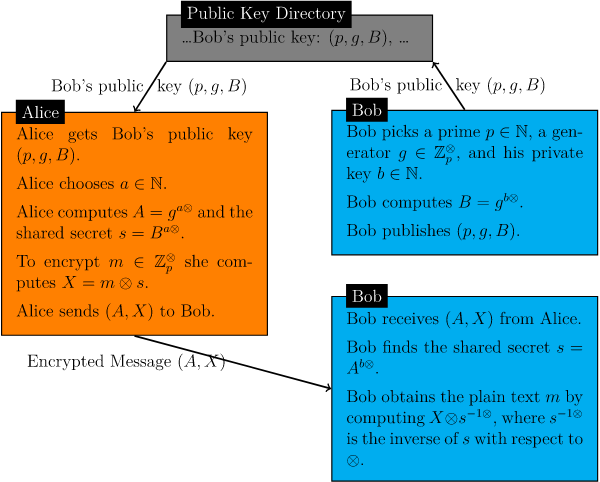
\includegraphics[width=15cm, height=12cm]{images/elgamal.png}



\section{Przykład działania}
\begin{comment}
\begin{enumerate}
    \item Generowanie Klucza przez Boba
    \begin{enumerate}
        \item weźmy liczbę $p=29$ i $g=2$
        \item weźmy $b=5$ jako klucz prywatny
        \item obliczmy $B=2^{5\otimes} = (2^{5}\,mod\,29=32\,mod\,29=3$
        \item publikujemy klucz składający się z $(p=29, g=2, B=3)$
    \end{enumerate}
    \item Szyfrowanie przez Alice\\
    Alice chce wysłać zaszyfrowaną wiadomość $m = 6$ do Boba
    \begin{enumerate}
        \item Alice dostaje od Boba $p=29, g=2, B=3$ z klucza publicznego
        \item wybieramy klucz prywatny a=4
        \item oblicza wspólny klucz prywatny $s=B^{a\otimes}=3^{4\otimes}= (3^{4}\,mod\,29=81\,mod\,29=23$
        \item obliczamy $A = g^{a} = 2^{4} = 16$
        \item szyfrujemy wiadomość $m=6$ jako $X = m\otimess=6\otimes23=138\,mod\,29=22$
        \item wysyłamy $(A, X) = (16, 22)$ do Boba
    \end{enumerate}
    \item Deszyfrowanie przez Boba\\
    Bob używa $A$ oraz swojego prywatnego klucza $b$, żeby rozszyfrować wiadomość
    \begin{enumerate}
        \item obliczamy wspólny klucz prywatny 
        \[ s=A^{b}\otimes = 16^{5\otimes}= 16^{4\otimes}\otimes16=(16^{2\otimes)^{2\otimes}}=\]
        \[=24^{2\otimes}\otimes16=25\otimes16=400\,mod\,29=23
        \]
        \item odwracamy $s^{-1\otimes} = 24$ z $s=23$ w $(\mathbb{Z}^{\otimes}_{29}, \otimes)$. 
        \item rozszyfrowujemy wiadomość przy obliczaniu $X\otimes s^{-1\otimes}=22\otimes24=528\,mod\,29 = 6$, czyli to co wysłała Alice
    \end{enumerate}
\end{enumerate}
\end{comment}

\begin{enumerate}
    \item Bob: klucz publiczny $(p, g, B)$, klucz publiczny $d$
    \begin{enumerate}
        \item Posiada:
    
        \begin{enumerate}
            \item Liczba pierwsza powinna mieć około 300 znaków, ale dla przykładu będzie ona mała \[p=13\]
            \item generator - liczba pierwotna dla powyższej liczby pierwszej\[g = 2\]
            \item $NWD(p,g)$ musi wynosić 1, aby operacja została wykonana
            \item sekretna liczba d musi spełniać warunek $(2\leq d\leq p-2)$ \[d=3\]
        \end{enumerate}
        \item Obliczenia:
        \begin{enumerate}
            \item \[B=g^{d}\,mod\, p \rightarrow B=2^{3}\,mod\,13 \rightarrow B=3\]
        \end{enumerate}
    
    \end{enumerate}
    \item Alice:
    \begin{enumerate}
        \item Posiada:
        \begin{enumerate}
            \item sekretna wiadomość, która jest mniejsza od $p$ \[m=4\]
            \item losowa liczba \[k=7\]
        \end{enumerate}
        \item Obliczenia:
        \begin{enumerate}
            \item \begin{gather}
                y_{1}=g^{k}\,mod\, p \rightarrow 2^{7}\,mod\,13=128\,mod\,13\rightarrowy_{1}=11
            \end{gather} 
            \item \begin{gather}
                y_{2}=me^{k}\,mod\, p\rightarrow(4*8^{7})\,mod\,13 \end{gather}
               \[ =(4*2097152)\,mod\,13=8388608\,mod\,13\rightarrow y_{2}=7\]
            
        \end{enumerate}
     \item Proces wysyłania wiadomości od Alice do Boba:
     \begin{enumerate}
         \item \[(y_{2}*y_{1}^{d})^{-1}\,mod\,p\]
         \item \[(7*11^{3})^{-1}\,mod\,13\]
         \item \[(7*8)\,mod\,13\]
         \item \[56\,mod\,13=4\]
     \end{enumerate}
    \end{enumerate}
\end{enumerate}
\section{Implementacja w języku Python}
\begin{enumerate}
    \item Generowanie klucza:\\
    \begin{python}
    #For key generation i.e. large random number
    def gen_key(q):
        key= random.randint(pow(10,20),q)
        while gcd(q,key)!=1:
            key=random.randint(pow(10,20),q)
        return key
    \end{python}
    \item Szyfrowanie\\
    \begin{python}
    #For asymetric encryption
    def encryption(msg,q,h,g):
        ct=[]
        k=gen_key(q)
        s=power(h,k,q)
        p=power(g,k,q)
        for i in range(0,len(msg)):
            ct.append(msg[i])
        print("g^k used= ",p)
        print("g^ak used= ",s)
        for i in range(0,len(ct)):
            ct[i]=s*ord(ct[i])
        return ct,p
    \end{python}
    \item Deszyfrowanie\\
    \begin{python}
    #For asymetric encryption
    def encryption(msg,q,h,g):
        ct=[]
        k=gen_key(q)
        s=power(h,k,q)
        p=power(g,k,q)
        for i in range(0,len(msg)):
            ct.append(msg[i])
        print("g^k used= ",p)
        print("g^ak used= ",s)
        for i in range(0,len(ct)):
            ct[i]=s*ord(ct[i])
        return ct,p
    \end{python}
\end{enumerate}
\section{Program w pythonie}
\pythonexternal{elgamal.py}
\begin{comment}
\section{Przykładowe ataki}
ElGamal, jak każdy inny sposób szyfrowania, posiada pewne schematy ataków na niego. Poniżej przedstawiono dwa z nich:meet-in-the-middle oraz Two Table
\begin{enumerate}
    \item Meet-in-the-middle attack\\
    Ten przypadek powstaje, gdy atakujący przechwycił szyfrogram $(r, s)$ i zna klucz publiczny $(p,g,B)$, który został użyty do zaszyfrowania wiadomości. Użyta zostaje tutaj tylko część druga szyfrogramu $s=mB^{k}$. Atak przebiega następująco:
    \begin{enumerate}
        \item Jedną z zalet ElGamala jest niedeterminizm. Jednakże niedeterministyczne wyrażenie $y^{k}$ ma stopień podziału $n$, więc jeżeli podniesiemy $s = my^{k}$ do potęgi $n$ to wyeliminujemy $y^{k}$:
        \[s^{n}=m^{n}(y^{k})^{n}=m^{n}(g^{xk})^{n}=m^{n}(g^{n})^{kx}=m^{n}\]
        \item Jednym z możliwych ataków jest zastosowanie brute force  na wiadomości $m'$ tak, że $m'^{n}=s^{n}$. Jednakże takie poszukiwania mogą zająć sporo czasu, dlatego wprowadzamy inne metody. Ograniczamy szukanie wiadomości $m'$, która możezostac sfaktoryzowana jak 
    \end{enumerate}
    
\end{enumerate}
\end{comment}

\section{Bibliografia}
\begin{enumerate}
    \item \href{https://sci-hub.se/https://dl.acm.org/doi/abs/10.1109/TIT.1985.1057074}{A Public Key Cryptosystem and a Signature
Scheme Based on Discrete Logarithms, 
TAHER ELGAMAL}
\item \href{https://minyak128.medium.com/elgamal-encryption-explained-38e9efda1a0f}{Implementacja algorytmu w Pythonie}
\item \href{https://mathstats.uncg.edu/sites/pauli/112/HTML/secelgamal.html}{Przykład zastosowania algorytmu}
\item \href{https://www.youtube.com/watch?v=nSTwr8rPfZk}{Wyjaśnienie wizualne działania}
\item \href{https://dr.lib.iastate.edu/server/api/core/bitstreams/112b99bf-add2-49aa-9cd5-b0be47948769/content}{Implementing several attacks on plain ElGamal encryption by Bryce Allen}
\item \href{sss}{sss}
\end{enumerate}
\end{document}
